\section{Method}
\label{sec:methods}

DEGST trains a sparse network in a single run. After a short dense warm-up, a sparse mask is initialised, and every $\Delta T$ iterations a fraction of the active weights is dropped according to an entropy-weighted score and replaced by the same number of inactive weights with the largest gradient. The loop is the one of RigL \cite{evci2020rigging}; the drop score and the mask initialisation are what DEGST changes (Algorithm~\ref{alg:degst}, Fig.~\ref{fig:framework}). Sections~\ref{sec:degst-s} and~\ref{sec:hybrid} extend the same entropy estimate to channels.

\begin{figure}
    \centering
    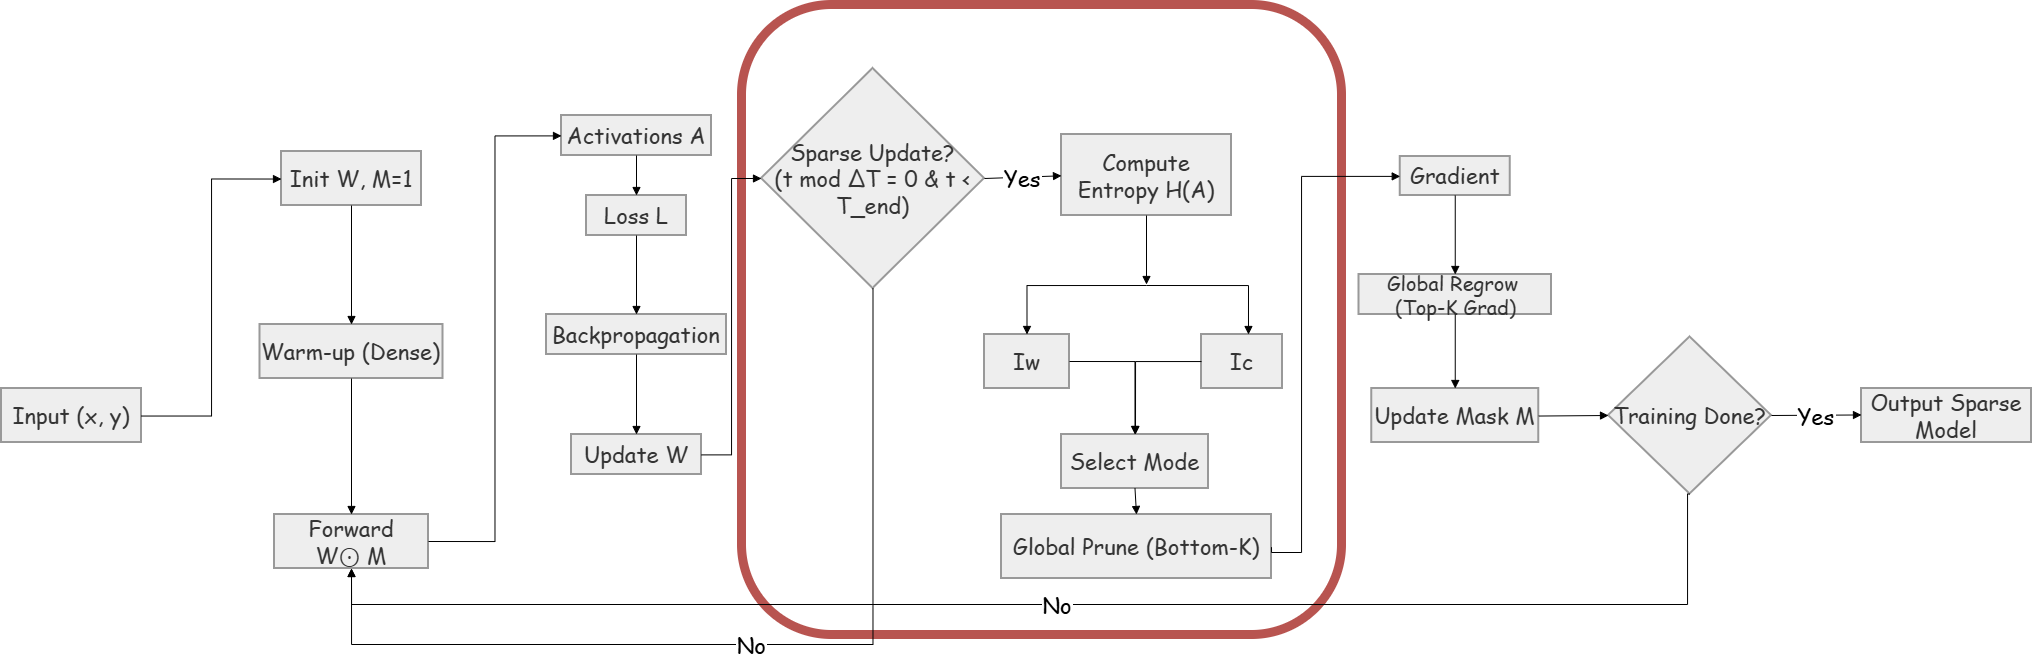
\includegraphics[width=1\linewidth]{Figures/Pipeline_highlight.png}
    \caption{DEGST training loop. After a dense warm-up, the entropy-guided branch (highlighted) runs every $\Delta T$ iterations until $T_{\text{end}}$: activation entropy is estimated from recent training batches and turned into weight-level ($I_w$) or channel-level ($I_c$) scores, the lowest-scoring active elements are dropped globally, and the same number of inactive elements with the largest gradient are regrown.}
    \label{fig:framework}
\end{figure}

\subsection{Notation and sparsity budget}

Let $W$ collect the weights of all convolutional and linear layers, $N=|W|$, and let $M\in\{0,1\}^{N}$ be a binary mask. The network computes with $W\odot M$ and is trained on the usual empirical risk. Throughout the paper, the \emph{sparsity} of a model is
\begin{equation}
S = 1 - \frac{\#\{\text{non-zero conv/linear weights of the final model}\}}{N},
\label{eq:sparsity}
\end{equation}
where $N$ always refers to the \emph{dense} model. Channels that are removed physically count as zeros. All methods, whether unstructured, structured or hybrid, are compared at the same $S$ and therefore keep the same number of weights. BatchNorm parameters are excluded from $N$; their count is reported separately.

\subsection{Activation entropy}

For a prunable layer $l$ with input tensor $A^{(l)}\in\mathbb{R}^{n\times C\times H\times W}$, we treat the $nHW$ values of input channel $c$ in a mini-batch as samples of a scalar random variable. Its range $[\min, \max]$ in that mini-batch is divided into $B$ equal-width bins. With $p_k$ the fraction of values that fall into bin $k$,
\begin{equation}
H^{(l)}_c = -\sum_{k=1}^{B} p_k \log (p_k + \epsilon),
\label{eq:entropy}
\end{equation}
with $B=30$ and $\epsilon=10^{-8}$. A channel that is constant over the batch has $H=0$, and the maximum is $\log B$. The estimate is taken from the last $K=4$ \emph{training} mini-batches before each topology update, with forward hooks, so no additional forward passes are needed. The $K$ values are aggregated by their mean (the median is evaluated in Sec.~\ref{sec:sensitivity}). For linear layers the samples are the $n$ values of each input feature.

A weight $w$ of layer $l$ reads exactly one input channel $c(w)$. For a grouped convolution with $G$ groups, output channel $o$ and in-group index $i$ read channel $\lfloor o/(C_{\text{out}}/G)\rfloor\cdot C_{\text{in}}/G + i$. The weight therefore inherits $H(w) := H^{(l)}_{c(w)}$ (Fig.~\ref{fig:entropy}).

\begin{figure}
    \centering
    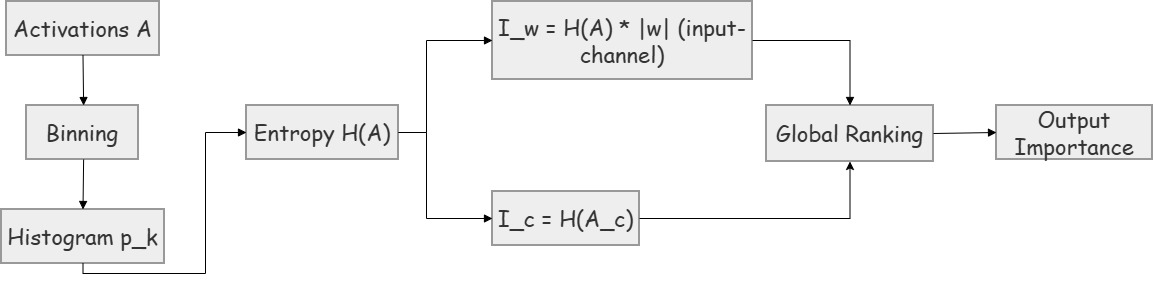
\includegraphics[width=0.75\linewidth]{Figures/Fig.2.jpg}
    \caption{Entropy-guided importance. Activations of each input channel are binned into a histogram, whose entropy is assigned to every weight that reads that channel ($I_w = H(A)\cdot|w|$). For channel pruning, the entropy of a channel's normalised output gives $I_c$. Both scores are ranked globally.}
    \label{fig:entropy}
\end{figure}

\paragraph{What entropy does and does not measure.}
Low $H$ means the input channel takes few distinct values over the data, for example a ReLU channel that is almost always zero or a saturated one. A weight reading such a channel acts almost like a bias, which motivates down-weighting it. However, $H$ is a property of the input distribution, not of the loss. It does not estimate how much the loss increases when the weight is removed, which is the quantity Taylor or Fisher saliencies approximate \cite{molchanov2019importance,theis2018faster}. Whether entropy helps is therefore an empirical question, and Sec.~\ref{sec:c0} answers it with an ablation.

\subsection{DEGST: entropy-weighted drop, gradient regrowth}
\label{sec:degst}

\paragraph{Scores.} The drop score of an active weight is
\begin{equation}
I_w = H(w)\cdot |w|.
\label{eq:iw}
\end{equation}
In the ablation of Sec.~\ref{sec:c0}, this score is replaced by $|w|$ (configuration A, the RigL drop criterion) or by $H(w)$ alone (configuration B), with everything else unchanged.

\paragraph{Mask initialisation.} The network is trained densely for $T_w$ epochs. The mask is then set by keeping the $(1-S)N$ weights with the largest $I_w$, ranked globally across layers.

\paragraph{Prune and regrow.} At every update step $t\in(T_w, T_{\text{end}}]$ with $t \bmod \Delta T = 0$, a fraction
\begin{equation}
\alpha_t = \frac{\alpha}{2}\left(1+\cos\frac{\pi (t-T_w)}{T_{\text{end}}-T_w}\right)
\label{eq:alpha}
\end{equation}
of the currently active weights is updated \cite{evci2020rigging}. The $k=\lfloor \alpha_t\, \|M\|_0\rfloor$ active weights with the smallest $I_w$ are dropped. The ranking is global, but the top 1\% of each layer's active weights are exempt so that no layer is disconnected. The same number of weights that were inactive before the update are regrown, choosing those with the largest dense gradient magnitude $|\partial\mathcal{L}/\partial w|$ on the current mini-batch. Regrown weights start at zero, and the momentum of every changed position is reset. Between updates, gradients of inactive weights are zeroed before the optimiser step, so the sparsity stays exactly $S$. Ties are broken by parameter index (stable sort), which makes the update deterministic given the scores.

\paragraph{Global versus per-layer allocation.} Because the ranking is global, the per-layer density is not fixed in advance: it emerges from the scores. Global magnitude-type rankings keep proportionally more weights in early layers, which operate at high spatial resolution. At a given $S$, they therefore remove fewer FLOPs than a layer-uniform allocation. This is why Sec.~\ref{sec:results} compares methods at equal FLOPs as well as at equal $S$.

\begin{algorithm}
\caption{DEGST (unstructured)}
\label{alg:degst}
\begin{algorithmic}[1]
\Require data $\mathcal{D}$, weights $W$, target sparsity $S$, warm-up $T_w$, interval $\Delta T$, end $T_{\text{end}}$, update fraction $\alpha$
\State $M \gets \mathbf{1}$
\For{$t = 1,\dots,T$}
\State forward with $W\odot M$ \Comment{hooks record $H^{(l)}_c$ if an update is due within $K$ steps}
\State backward: dense gradient $g$
\If{$t = T_w$}
\State $M \gets$ top-$(1-S)N$ of $I_w = H\cdot|w|$ (global)
\ElsIf{$T_w < t \le T_{\text{end}}$ \textbf{and} $t \bmod \Delta T = 0$}
\State $k \gets \lfloor \alpha_t \|M\|_0 \rfloor$ \Comment{Eq.~(\ref{eq:alpha})}
\State drop the $k$ active weights with smallest $I_w$ (global, per-layer floor)
\State grow the $k$ previously inactive weights with largest $|g|$; set them to $0$; reset their momentum
\EndIf
\State $g \gets g \odot M$; SGD step; $W \gets W\odot M$
\EndFor
\State \Return $W\odot M$
\end{algorithmic}
\end{algorithm}

\subsection{DEGST-S: channel-level prune and regrow}
\label{sec:degst-s}

\paragraph{Coupled channel groups.} In residual networks, the channels of the residual stream are shared by the stem, by the last convolution of every block and by the shortcut projections. In MobileNetV2, the expansion and depthwise convolutions are coupled as well. Such channels can only be removed together. We obtain the coupled groups from DepGraph \cite{fang2023depgraph}: ResNet-18 has 12 groups and MobileNetV2 has 26. The classifier's output is never pruned.

\paragraph{Gates.} Each group $g$ carries a binary gate vector that multiplies the outputs of all BatchNorm layers in the group. A zero gate silences the channel everywhere it appears, so the gated network is exactly equivalent to the network with that channel removed. We verified that the outputs agree to $10^{-7}$ after physical removal. The gate also provides a regrowth signal: its gradient $\partial\mathcal{L}/\partial g_c$ is defined for silenced channels, which lets channels be regrown in the same way that RigL regrows weights.

\paragraph{Channel score and schedule.} The channel score $I_c$ is the entropy (Eq.~\ref{eq:entropy}) of the channel's BatchNorm output, averaged over the BatchNorm layers of its group. The weight budget follows the cubic schedule of \cite{zhu2017prune}, from $N$ at $T_w$ to $(1-S)N$ at $T_{\text{end}}$. At each update, a fraction $\alpha_t$ of the active channels with the smallest $I_c$ is swapped for the inactive channels with the largest $|\partial\mathcal{L}/\partial g_c|$ accumulated since the previous update. The lowest-$I_c$ channels are then silenced, in global order, until the weight count computed for the resulting architecture reaches the scheduled budget. Every group keeps at least 5\% of its channels. At $T_{\text{end}}$ the silenced channels are removed physically, and training continues on the compact dense model. The final weight count matches the budget to within one channel.

\subsection{Hybrid sparsity}
\label{sec:hybrid}

The hybrid variant splits one budget $S$ between the two levels. The structured stage runs DEGST-S towards a weight sparsity $\beta S$ ($\beta=0.5$ by default) and removes the channels physically at the midpoint of the update window, $T_{\text{mid}}=(T_w+T_{\text{end}})/2$. Let $N_c$ be the weight count of the compact model. Unstructured DEGST then runs inside the compact model from $T_{\text{mid}}$ to $T_{\text{end}}$ at the inner sparsity
\begin{equation}
s_u = 1 - (1-S)\frac{N}{N_c},
\end{equation}
so that the overall sparsity (Eq.~\ref{eq:sparsity}) equals $S$ exactly. The channel budget therefore scales with the target, and the executed FLOPs reflect only the structured part.

\subsection{Cost}

Masking and scoring are element-wise, and each update performs one global sort of the active scores. The histograms (Eq.~\ref{eq:entropy}) are linear in the number of activations of the $K$ recorded batches per $\Delta T$ iterations. Section~\ref{sec:cost} reports the measured wall-clock overhead of each part. As in all mask-based sparse training, the forward and backward passes are dense, so DEGST does not reduce training FLOPs.
